\chapter{Motivation}\label{ch:motivation}
 This chapter accounts for the motivation behind source extraction from an Electroencephalography (EEG). The concept of EEG is introduced along with current applications. The potential and importance of source extraction are considered and related to the hearing aid industry. The commonly applied mathematical model for EEG measurements is presented. Currently applied methods for source extraction are considered leading to a presentation of the current state of the art methods which succeeds to overcome the limitations of previous methods. Lastly the objective of this thesis is specified.          

%%This chapter examines existing literature concerning source recovery from Electroencephalography (EEG) measurements. 
%%At first a motivation for the source recovery problem is given, considering the application within the hearing aid industry. 
%%Further, the state of the art methods are presented followed by a description of the contribution proposed in this thesis.

\section{Introduction to EEG Measurements}\label{sec:EEG}
EEG is an imaging technique used within the medical field. EEG is measuring electric signals on the scalp, caused by brain activity. 
The human central nerve system consist of various nerve cells connecting the neurons within the brain. Nerve cells respond to certain stimuli, for instance a physical stimuli, and transmit informations between neurons.
Generally speaking these activities induce local currents that are transferred throughout the nerve system. 
Several nearby simultaneous activations result in local potential fields, referred to as one signal \textit{source}\cite{EEGsignalprocessing}. 
EEG measurements are provided by a number of metal electrodes, referred to as sensors, carefully placed on the human scalp. 
Each sensor reads the present electrical signals over time.
For the source signal to reach a sensor it has to penetrate the skull, skin and several other thin layers of biological tissue. 
This causes an unknown distortion and reduction of a signal.
It is most likely that the measurement of one sensor is a sum of multiple signals from different sources.
Nor is the range of a single sensor separated from the other sensors. 
Thus the same signal can easily be measured by two or more sensors.
The process of distorsion and mixing of signals is called volume conduction \cite[p. 68]{EEGsignalprocessing} \cite{Van2019}. 
From this it is clarified that EEG measurements  
is a mixture of fluctuating electrical signals originating from brain activities. Due to the mixing and the nature of the signals the true number of sources is generally considered unknown\cite{EEGsignalprocessing}.  
Furthermore, EEG is a subject for interfering noise. Noise signals can occur in the measurements resulting from physical movement of e.g. eyes and jawbone \cite{fundamentalEEG}. The concept of volume conduction is sought illustrated on figure \ref{fig:volumeconduction}.

The source signals are classified within four groups according to the dominant frequency. 
The delta wave ($0.5-4$ Hz) is observed from infants and sleeping adults, the theta wave ($4-8$ Hz) is observed from children and sleeping adults, the alpha wave ($8-13$ Hz) is the most extensively studied brain rhythm, which is induced by an adult laying down with closed eyes. 
Lastly, the beta wave ($13-30$ Hz) is considered the normal brain wave for adults, associated with active thinking, active attention or solving concrete problems \cite[p. 11]{EEGsignalprocessing}. 
An example of EEG measurements within the four categories is illustrated by figure \ref{fig:EEG_example}.   

Generally, the distribution of EEG measurements of multiple sensors are considered multivariant Gaussian\todo{does this comply to the non-gaussian assumption of ICA?} \cite[p. 50]{EEGsignalprocessing}. Though the mean and covariance properties generally changes over time. Therefore EEG measurements are considered quasistationary i.e. stationary only within small intervals. This motivates the need for segmentation of the EEG measurements to achieve signals with similar characteristics. 

\begin{figure}[H]
    \begin{minipage}[t]{.45\textwidth}
        \centering
        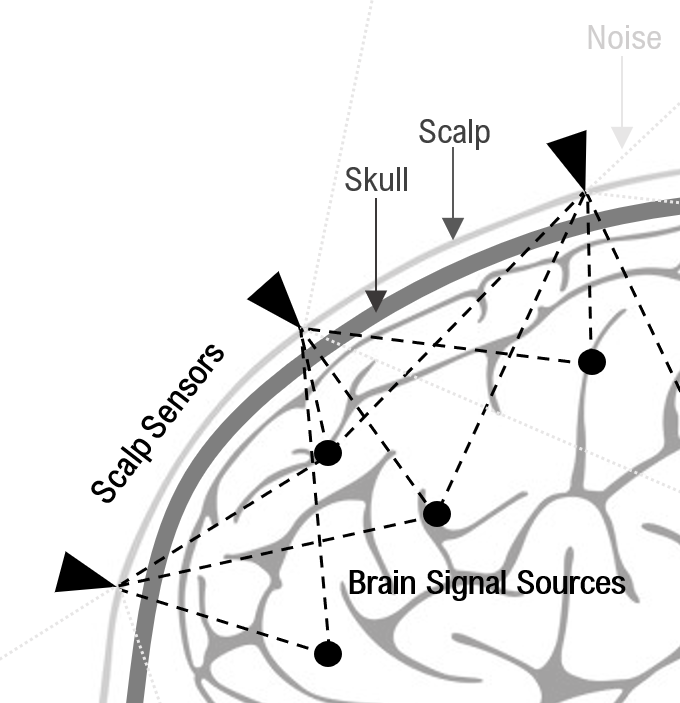
\includegraphics[width=\textwidth]{figures/EEG/volumeconduction.png}
        \caption{Illustration of volume conduction}\label{fig:volumeconduction}
    \end{minipage} 
    \hfill
    \begin{minipage}[t]{.45\textwidth}
        \centering
        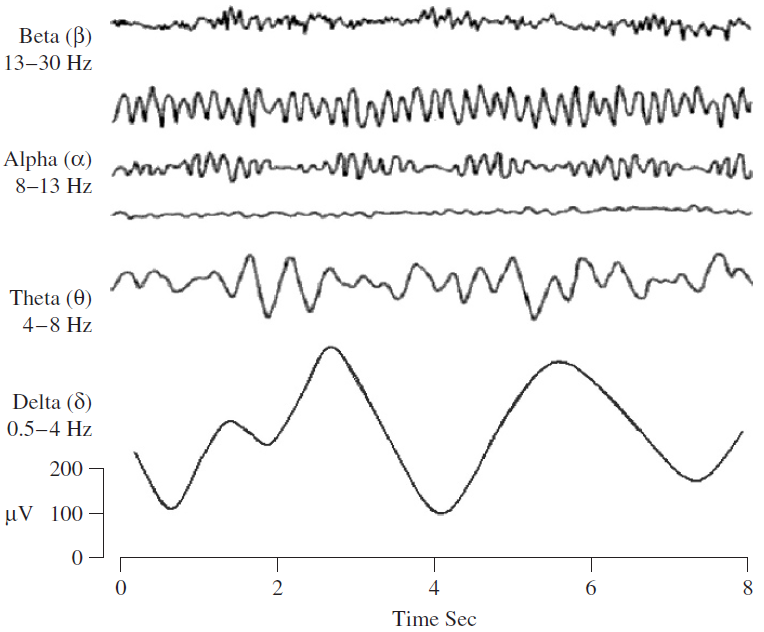
\includegraphics[width=\textwidth]{figures/EEG/EEG_example.png}
        \caption{Example of time dependent EEG measurements within the four defined categories, source: \cite{EEGsignalprocessing}}\label{fig:EEG_example}
    \end{minipage}
\end{figure}

\subsection{Application}
EEG performed on humans and animals have a great number of applications with both clinical and research purposes. 
Examples of clinical applications covers diagnosis and management of neurological disorders such as epilepsy and monitor alertness regarding coma or brain death.
EEG capitalizes on the procedure being non-invasive and fast.
Neural activity can be measured within fractions of a second after a stimuli has been provided. 
These advantages contributes to the wide range of applications within research of the neural processes involved in or resulting from actions, emotions or  cognition. Today such neural research are use in many different fields\cite[p. 4]{fundamentalEEG}.
% such as neuromarketing, biofeedback(optimisation of learning) and brain computer interface.  
The hearing aid industry is one example where this research is highly prioritized. 
At Eriksholm research center, which is a part of the hearing aid manufacturer Oticon, cognitive hearing science is a research area within fast development \cite{Weberik}. 
One main purpose at Eriksholm is to make it possible for a hearing aid to identify the user-intended sound source from real time EEG measurements and thereby exclude noise from elsewhere \cite{Emina2019} \cite{Bech2018}. 
It is essentially the well known but unsolved cocktail problem which is sought improved by use of EEG. 
This is where EEG and occasionally so called in-ear EEG is interesting. In conjunction with the technology of beamforming it is possible for a hearing aid to receive only signals from a specific direction. 

Over the past two decades, functional integration has become an area of interest regarding EEG research \cite{Friston2011}. 
Within neurobiology functional integration refers to the study of the correlation among activities in different regions of the brain. 
In other words, how do different parts of the brain work together to process information and conduct a response \cite{Friston2002}.     
For this purpose separation and localization of the original sources which contribute to the EEG measurement is of interest. 
An article from 2016 \cite{Van2019} points out the importance of performing analysis regarding functional integration at source level rather than at EEG level. 
It is argued through experiments that analysis at EEG level does not allow interpretations about the interaction between sources. 
This emphasize a potential for improving results within a wide range of EEG research, if the original active sources can be extracted from a specific EEG measurements.    

%     
%However, the focus of this research is the correlation between EEG measurements and the sound source rather than localization of the activated source from the EEG \cite{Emina2019}. 
%Hence a source localization approach could potentially be of interest regarding hearing aids in order to improve the results.
%(Furthermore, a real-time application to provide feedback from EEG measurements would be essential.)\todo{?}. 


\subsection{Modelling}
Consider the issue of extracting the activated sources from EEG measurements. A known approach is to model the observed data by a linear system 
\begin{align*}
\mathbf{y} = \mathbf{Ax}.
\end{align*}
The vector $\mathbf{y} \in \mathbb{R}^{M}$ is the EEG measurement of one time sample containing $M$ sensor measurements. $\mathbf{x} \in \mathbb{R}^{N}$ is the corresponding $N$ sources within the brain. 
The non-zero entries of $\textbf{x}$ represent the active sources at the time of the measurement. 
$\mathbf{A} \in \mathbb{R}^{M \times N}$ is an unknown projection/transformation(?) matrix, also referred to as the mixing matrix resembling the volume conduction. 
The $i^{th}$ column of $\mathbf{A}$ represents the relative projection weights from the $i^{th}$ source to every sensor \cite{phd2015}. 
Representing one time sample the linear system is in general referred to as a single measurement vector model. 
It it only the measurement vector $\textbf{y}$ that is known hence it is not possible to solve the linear system with respect to $\textbf{x}$ using basic linear algebra.   
The task in this case is to identify both $\mathbf{A}$ and then $\mathbf{x}$, given the measurement vector $\mathbf{y}$. This problem is referred to as the inverse problem of EEG. 
Finding $\textbf{x}$ from the inverse problem is referred to as source separation and localization. Separation is to find the signal of each active source and localization is to place each active source signal at the right position within the source vector of dimension $N$, where $N$ is the maximum number of sources to be active.      

Independent Component Analysis (ICA) is one commonly applied method to solve the inverse problem of EEG \cite{Scott1996}, \cite{Scott1997}. ICA is a technique to find the matrix $A$ such that the column wise elements of $X$ is statistically independent. Thus statistical independence between the active sources is the essential assumption, which in the case of EEG are considered valid due to the volume conduction being effectively instantaneous\cite[p. 3]{Scott1997}. 
Application of ICA has shown great results regarding source separation of high-density EEG. 
However, a significant flaw to this method is that the EEG measurements are only separated into a number of sources that is equal to or less than the number of sensors \cite{Balkan2015}.
Meaning that the EEG inverse problem can not be solved when  it forms an under-determined system, which is the case when the maximum number of unknown sources $N$ exceeds the number of sensors $M$. 
Such assumption undermines the reliability and usability of ICA, as the number of active sources easily exceed the number of sensors \cite{phd2015}. 
This is especially a drawback when low-density EEG are considered. Low-density EEG measurements are collected from equipment with less than 32 sensors, increasing the changes of $M$ being less that $N$. 
However, improved capabilities of low-density EEG devices are desirable due to their relative low cost, mobility and ease to use. 

This argues the importance of considering the inverse problem of EEG in the under-determined case where $N>M$. In the next section existing work considering the under-determined inverse problem of EEG is investigated further. 

\section{Related Work and Our Objective} 
As mentioned above ICA is a solid method for source separation in the case where separation into a number of sources equal to the number of sensors is adequate. The issue occurs in cases where the number of sources $N$ exceeds the number of sensors $M$.  
To overcome this issue an extension of ICA was suggested, referred to as the ICA mixture model \cite{Balkan2015}.
Instead of identifying one overcomplete mixing matrix $\mathbf{A} \in \mathbb{R}^{M \times N}$ this approach learns $N_{\text{model}}$ different mixing matrices $\mathbf{A}_i \in \mathbb{R}^{M\times M}$, to make computations more tractable. 
This method was further adapted into the Adaptive Mixture ICA (AMICA) which showed successful results regarding identification of more sources than sensors \cite{Palmer2008}. 
However, these successful results relies on the assumption that no more than $M$ out of $N$ possible sources is simultaneously active. That is explicit that the source vector of dimension $N$ has at most $M$ non-zero entries.
This assumption is still an essential limitation to the frame work, especially when considering low-density EEG. 
Other types of ICA algorithms for under-determined systems have been proposed, without overcoming the limitation of jointly active sources exceeding the number of sensors.
%One is the Restricted ICA (RICA), an efficient method used for unsupervised learning in neural networks \cite{Le2011}.\\ 

In 2015 O. Balkan et. al. suggested a new approach also targeting the identification of more active sources than sensors regarding EEG measurements. One method is proposed for learning $\textbf{A}$ from $\textbf{y}$\cite{Balkan2015} and a different method is proposed for finding $\textbf{x}$ given $\textbf{y}$ and $\textbf{A}$\cite{Balkan2014}.

To learn $\textbf{A}$ the suggested method, referred to as Cov-DL, is a covariance-domain based dictionary learning algorithm. 
The method is based upon theory of dictionary learning and compressive sensing. Which dictates a framework for solving an under-determined system when $\textbf{x}$ contains a sufficiently amount of zeros. 
This is similar to the constraint of ICA.  However, to overcome this the point is to transfer the EEG measurements into the covariance domain. In the covariance domain a higher dimensionality can be achieved compared to the original EEG sensor domain with dimension $M$.
The transformation can be done when assuming a linear volume conduction and uncorrelated sources.
As a result the theory of compressive sensing is found to  apply to the covariance domain, allowing to learn $\textbf{A}$ by dictionary learning -- even in the case where the active sources exceeds the number of measurements.

The Cov-DL algorithm stands out from other straight forward dictionary learning methods as it does not relay on the sparsity of active sources\todo{is it okay to mention sparsity here for the first time?}. This is an essential advantage when low-density EEG is considered. 
Cov-DL was tested and found to outperform AMICA \cite{Balkan2015}.  
As mentioned, the Cov-DL algorithm only learns the mixing matrix $\mathbf{A}$, resembling the volume conduction.

For the purpose of recovering $\textbf{x}$, from $\textbf{y}$ and $\textbf{A}$, a multiple measurement sparse Bayesian learning (M-SBL) algorithm is proposed. This method is also targeting the case of more active sources than sensors.\todo{yderligere beskrivelse nødvedig? eller fjerne lidt fra Cov måske, da det samme lidt kommer i kap 3?}
The method was proven to outperform the previously used algorithms, even when the defined recovery conditions regarding the found mixing matrix $\textbf{A}$ was not fulfilled\cite{Balkan2014}.

One drawback, which is not fully covered in the referred literature, is that the two methods rely on the number of active sources being known. 
In practise this is not the case. 
Hence an estimation of the number of active sources has to be considered for the algorithm to be useful in practice. To address this issue a simple approach is to optimise the result with respect to the number active source, provided that some prior assumption of the expected result can be made.      
\\ \\
The two state of the art methods resulting in source separation and localization will make the foundation of this thesis. 
Our aim is to investigate and fully understand the two methods in order to implement and test a joint algorithm -- recovering the original sources $\textbf{x}$ from the measurements $\textbf{y}$, when the number of active sources exceeds the number of measurements. 
Secondary it is of interest to consider the practical application of the algorithm, for instance within a hearing aid as described in section \ref{sec:EEG}.  
%As described in section \ref{sec:EEG}  it is of interest to reduce the amount of energy it takes to listen to a specific sound source surrounded by noise.
%For this purpose we want to relate the found number of active sources to the level of concentration that the test person is experiencing. 
As mentioned, the number of active sources is in general unknown in practise thus it is first of all an estimation of the number of active sources which is of interest for practical use of the algorithm. 
For this we want to investigate whether it is possible to estimate the number of active sources, through optimization.   
 


 
